%%%%%%%%%%%%%%%%%%%%%%%%%%%%%%%%%%%%%%%%%%%%%%%%%%%%%
%% Use a minimum font size of 12pt and specify a4paper
%% for ease of display and printing in the UK
%%%%%%%%%%%%%%%%%%%%%%%%%%%%%%%%%%%%%%%%%%%%%%%%%%%%%
\documentclass[12pt,a4paper]{article}

%%%%%%%%%%%%%%%%%%%%%%%%%%%%%%%%%%%%%%%%%%%%%%%%%%%%%
%% Geometry package to change margins etc.
%%%%%%%%%%%%%%%%%%%%%%%%%%%%%%%%%%%%%%%%%%%%%%%%%%%%% 
\usepackage[a4paper,margin=2.5cm]{geometry}

%%%%%%%%%%%%%%%%%%%%%%%%%%%%%%%%%%%%%%%%%%%%%%%%%%%%%
%% Babel package to specify English typographical 
%% rules, and hyphenation patterns
%%%%%%%%%%%%%%%%%%%%%%%%%%%%%%%%%%%%%%%%%%%%%%%%%%%%%
\usepackage[english]{babel}

%%%%%%%%%%%%%%%%%%%%%%%%%%%%%%%%%%%%%%%%%%%%%%%%%%%%%
%% T1 font encoding to ensure characters with accents 
%% and other non-ascii characters can be correctly 
%% searched, copied and pasted in the PDF output. Also 
%% enables hyphenation of words containing letters 
%% with accents.
%%
%% Note, you should have cm-super installed otherwise
%% computer modern fonts will be bitmaps. 
%% If this is a problem then move this command inside
%% a clearprint toggle below. 
%%%%%%%%%%%%%%%%%%%%%%%%%%%%%%%%%%%%%%%%%%%%%%%%%%%%%
\usepackage[T1]{fontenc}

%%%%%%%%%%%%%%%%%%%%%%%%%%%%%%%%%%%%%%%%%%%%%%%%%%%%%
%% This is the master for 3 document formats.
%% We DO NOT support compiling via latex-dvips-ps2pdf. 
%% If you wish to use diagrams which rely on this 
%% then these should be produced as standalone figures 
%% in PDF and svg formats and included in the LaTeX
%% via the graphicx package.
%%
%% Standard print: Compiled via pdflatex. You can 
%% style how you provided you can compile the other
%% formats.
%% 
%% Clearprint: Compiled via pdflatex. 
%%
%% Accessible web pages via TeX4ht with MathJax
%% as the renderer: for zoom, magnification, text to 
%% speech (TextHelp Read & Write), screenreaders 
%% (NVDA, JAWS 16+, ChromeVox, other Aria aware), 
%% electronic braille (NVDA), also good on small 
%% screens. 
\usepackage{etoolbox}
\newtoggle{clearprint}
\newtoggle{web}
%% The below uses the make file to determine which 
%% format to compile. Please note that compilation 
%% requires a post-2009 version of etoolbox and, for 
%% the web format, a working copy of TeX4ht. 
%% Using the makefile is the recommended compilation 
%% method as this will produce a single zip containing
%% the web format for you. 
\togglefalse{clearprint}\toggletrue{web}

%% If you are NOT using the make file you may 
%% uncomment one of the below:
%%
%% Standard print PDF. Compiled via pdflatex:
%\togglefalse{clearprint}\togglefalse{web}
%%
%% Clear print PDF. Compiled via pdflatex: 
%\toggletrue{clearprint}\togglefalse{web}
%%
%%Accessible web format. Requires TeX4ht - see 
%% make file for commands to run: 
%\togglefalse{clearprint}\toggletrue{web}
%%%%%%%%%%%%%%%%%%%%%%%%%%%%%%%%%%%%%%%%%%%%%%%%%%%%%

%%%%%%%%%%%%%%%%%%%%%%%%%%%%%%%%%%%%%%%%%%%%%%%%%%%%%
%% Standard packages loaded.
%%%%%%%%%%%%%%%%%%%%%%%%%%%%%%%%%%%%%%%%%%%%%%%%%%%%%
%% Only graphicx and the picture environment can 
%% be used for graphics.  
\usepackage{amsmath,amssymb,amsfonts,amsthm}
\usepackage{hyperref} %% We rely on this
%%
%% Graphicx must be loaded whether used or not as 
%% TeX4ht compilation expects it.
%% EPS diagrams can be used directly from TeXLive 2015
%% onwards. Before this you will need to hand convert
%% to PDF. 
\usepackage{graphicx} %% We rely on this
\graphicspath{{./figures/}} 
%%%%%%%%%%%%%%%%%%%%%%%%%%%%%%%%%%%%%%%%%%%%%%%%%%%%%
%% Other packages may not work for this process.
%% See the second example for further packages. 
%%%%%%%%%%%%%%%%%%%%%%%%%%%%%%%%%%%%%%%%%%%%%%%%%%%%%
\usepackage{longtable}
\usepackage[mathscr]{eucal}
\usepackage{eufrak} 

%%%%%%%%%%%%%%%%%%%%%%%%%%%%%%%%%%%%%%%%%%%%%%%%%%%%%
%% Requirements for clearprint/web version
%%%%%%%%%%%%%%%%%%%%%%%%%%%%%%%%%%%%%%%%%%%%%%%%%%%%%
\ifboolexpr{togl {clearprint} or togl {web}}{
%% Change font to Helvetica and heavier verbatim font
\renewcommand{\familydefault}{phv}
\fontfamily{phv}\selectfont
\usepackage[scaled=0.95]{DejaVuSansMono}

%% Emphasis in bold only - add additional examples 
%% as per resource
\renewcommand{\em}{\bf}
\renewcommand{\textit}{\textbf}
\renewcommand{\emph}{\textbf}
\renewcommand{\it}{\bf }

%% Additional spacing - may not be honoured in 
%% web version
\setlength{\parindent}{0.0pt}
\setlength{\parskip}{1.0\baselineskip}
\renewcommand{\baselinestretch}{1.25}\selectfont
\mathsurround 0.2em
\setlength{\arraycolsep}{0.5cm}\renewcommand{\arraystretch}{1.25}
\addtolength{\jot}{0.5\baselineskip}
\sloppy
\allowdisplaybreaks 
}

%%%%%%%%%%%%%%%%%%%%%%%%%%%%%%%%%%%%%%%%%%%%%%%%%%%%%
%% To include code listings use the listings package. 
%% Also load spverbatim for a basic verbatim environment which can line break if needed
%%\usepackage{verbatim}
\usepackage{spverbatim}
\usepackage{listings} 
\lstloadlanguages{Matlab} %Other languages are available, see manual, you should select the correct language
\lstset{
basicstyle=\ttfamily, 
breaklines=true, 
columns=fixed 
}

%%%%%%%%%%%%%%%%%%%%%%%%%%%%%%%%%%%%%%%%%%%%%%%%%%%%%
%% Commands used to provide alternative text for 
%% diagrams for a screenreader user.
%% DO NOT remove the macros from the preamble even if
%% you are not using them as the web compilation 
%% expects them to be defined.
\newcommand{\nextalt}[1]{} 
\newcommand{\PICalt}[1]{{#1}} 
%%%%%%%%%%%%%%%%%%%%%%%%%%%%%%%%%%%%%%%%%%%%%%%%%%%%%

%%%%%%%%%%%%%%%%%%%%%%%%%%%%%%%%%%%%%%%%%%%%%%%%%%%%%
%% You can style your theorems etc. as you like but 
%% in clearprint and accessible web use a clearprint 
%% style to open up spacing, use bold for emphasis 
%% and to avoid large parts of text in italics. 
\ifboolexpr{togl {clearprint} or togl {web}}
{
\newtheoremstyle{clearprint}
{20pt}% space above
{3pt}% space below
{}% body font
{}% indent amount
{\bfseries}% theorem head font
{.\newline }% punctuation after theorem head
{1.0em}% space after theorem head
{}% theorem head spec, can be left empty meaning normal
\theoremstyle{clearprint}
\newenvironment{Proof}
{\noindent{\bf Proof.}\hspace*{1em}}% Begin
{\qed\par}% End
%% When redefining an environment it is vital that it has 
%% the same number of arguments as the original
\renewenvironment{proof}[1][\proofname]
{\noindent{\bf {#1}.}\hspace*{1em}}% Begin
{\qed\par}% End
}
%%%%%%%%%%%%%%%%%%%%%%%%%%%%%%%%%%%%%%%%%%%%%%%%%%%%%
%% Leave a blank line after this

%%%%%%%%%%%%%%%%%%%%%%%%%%%%%%%%%%%%%%%%%%%%%%%%%%%%%
%% In default style in standard print
\newtheorem{theorem}{Theorem}[section]
\newtheorem{corollary}[theorem]{Corollary}
%%%%%%%%%%%%%%%%%%%%%%%%%%%%%%%%%%%%%%%%%%%%%%%%%%%%%

%%%%%%%%%%%%%%%%%%%%%%%%%%%%%%%%%%%%%%%%%%%%%%%%%%%%%
%% Change to definition style for the standard print
\ifboolexpr{togl {clearprint} or togl {web}}
{\theoremstyle{clearprint}}
{\theoremstyle{definition}}
%% Leave a blank line after this

%%%%%%%%%%%%%%%%%%%%%%%%%%%%%%%%%%%%%%%%%%%%%%%%%%%%%
%% In definition style unless in clearprint
\newtheorem{definition}{Definition}[section]
%%%%%%%%%%%%%%%%%%%%%%%%%%%%%%%%%%%%%%%%%%%%%%%%%%%%%

%%%%%%%%%%%%%%%%%%%%%%%%%%%%%%%%%%%%%%%%%%%%%%%%%%%%%
%% Change to remark style for the standard print
\ifboolexpr{togl {clearprint} or togl {web}}
{\theoremstyle{clearprint}}
{\theoremstyle{remark}}
%% Leave a blank line after this

%%%%%%%%%%%%%%%%%%%%%%%%%%%%%%%%%%%%%%%%%%%%%%%%%%%%%
%% In remark style unless in clearprint
\newtheorem*{note}{Note}
%%%%%%%%%%%%%%%%%%%%%%%%%%%%%%%%%%%%%%%%%%%%%%%%%%%%%

%%%%%%%%%%%%%%%%%%%%%%%%%%%%%%%%%%%%%%%%%%%%%%%%%%%%%
%% Place any document specific commands here
\newcommand{\xsb}{x_{1}}
\newcommand{\xsp}{x^{2}}
\newcommand{\xsbnum}[1]{x_{#1}}
\newcommand{\boo}{\mathrm{boo}}
\newcommand{\End}{\mathrm{End}}

%%%%%%%%%%%%%%%%%%%%%%%%%%%%%%%%%%%%%%%%%%%%%%%%%%%%%
%% To enable 'faked' commuting diagrams
\newcommand{\mapright}[1]{{\stackrel{#1}{\longrightarrow}}}
\newcommand{\mapdown}[1]{\Big\downarrow{\scriptstyle{#1}}} 
\newcommand{\tab}{&}

%%%%%%%%%%%%%%%%%%%%%%%%%%%%%%%%%%%%%%%%%%%%%%%%%%%%%
%% Define front matter
\title{AMS stress test document}
\author{Emma Cliffe}

%%%%%%%%%%%%%%%%%%%%%%%%%%%%%%%%%%%%%%%%%%%%%%%%%%%%%
%% Ensure front matter and table of contents are 
%% page numbered separately from the body
%% Use headings style so that each page has a label
\ifboolexpr{togl {clearprint} or togl {web}}{
\pagestyle{headings}
\pagenumbering{roman}
}
%%%%%%%%%%%%%%%%%%%%%%%%%%%%%%%%%%%%%%%%%%%%%%%%%%%%%

%%%%%%%%%%%%%%%%%%%%%%%%%%%%%%%%%%%%%%%%%%%%%%%%%%%%%
%% End the preamble
\begin{document}

%%%%%%%%%%%%%%%%%%%%%%%%%%%%%%%%%%%%%%%%%%%%%%%%%%%%%
\maketitle

%%%%%%%%%%%%%%%%%%%%%%%%%%%%%%%%%%%%%%%%%%%%%%%%%%%%%
%% In longer documents place a newpage before the tables
%% You may not want all of the tables in all formats
%% \newpage 
\tableofcontents
\listoffigures
\listoftables
\newpage

%%%%%%%%%%%%%%%%%%%%%%%%%%%%%%%%%%%%%%%%%%%%%%%%%%%%%
%% Page numbering for the body of the document starts
\pagenumbering{arabic}
\setcounter{page}{1}
%%%%%%%%%%%%%%%%%%%%%%%%%%%%%%%%%%%%%%%%%%%%%%%%%%%%%

%%%%%%%%%%%%%%%%%%%%%%%%%%%%%%%%%%%%%%%%%%%%%%%%%%%%%
%% If a section/subsection/subsubsection is unnumbered
%% but it makes sense to add it to the table of 
%% contents for the web version then add contents
%% line by hand. 
\section*{Using this document}
\ifboolexpr{not (togl {web})}{\addcontentsline{toc}{section}{Using this document}}

This is the AMS \LaTeX~ test document compiled from \LaTeX~ into multiple formats:
\begin{itemize} 
\item \href{https://stem-enable.github.io/LaTeXtoPDFandMathJax-AMSStressTest/LaTeXtoPDFandMathJax-AMSStressTest-standard.pdf}{Standard print PDF}
\item \href{https://stem-enable.github.io/LaTeXtoPDFandMathJax-AMSStressTest/LaTeXtoPDFandMathJax-AMSStressTest-clear.pdf}{Clearer print PDF}
\item \href{https://stem-enable.github.io/LaTeXtoPDFandMathJax-AMSStressTest/}{Accessible web format}
\item \href{https://stem-enable.github.io/LaTeXtoPDFandMathJax-AMSStressTest/LaTeXtoPDFandMathJax-AMSStressTest.docx}{Accessible Word document}
\end{itemize}

The primary purpose of this document is to test parts of AMS \LaTeX~ with some additional packages under various transforms. The content of this document is {\bf not} a description of a transformable set of \LaTeX~which will certainly be smaller.  

\newpage


%%%%%%%%%%%%%%%%%%%%%%%%%%%%%%%%%%%%%%%%%%%%%%%%%%%%%
%% Start of AMS stress test
%%%%%%%%%%%%%%%%%%%%%%%%%%%%%%%%%%%%%%%%%%%%%%%%%%%%%

\section[Standard fonts and symbols]{Standard fonts and symbols}
\setcounter{equation}{0}

\noindent
A baseline of text which is a single line long in 12pt font with no indent applied.

\begin{center}
Centered text.
\end{center}

\begin{flushleft}
Flush left text.
\end{flushleft}

\begin{flushright}
Flush right text.
\end{flushright}

\noindent
A baseline of text which is a single line long in 12pt font with no indent applied.

Standard text. {\tiny Tiny text.} {\scriptsize Scriptsize text.} {\footnotesize Footnotesize text.} {\small Small text.} {\normalsize Normalsize text.} {\large large text.} {\Large Large text.} {\LARGE LARGE text.} {\huge huge text.} {\Huge Huge text.}

Standard text. \emph{Emphasized text}. \textrm{Roman text.} {\rm Roman inline.} \textsc{Small caps text.} {\sc Small caps inline} \texttt{Typewriter text.} {\tt Typewriter inline.} \textit{Italics text.} {\it Italics inline.} \textsf{Sans serif text.} {\sf San serif inline.} \textsl{Slant text.} {\sl Slant inline.}  \textbf{Bold text.} {\bf Bold inline.} \textbf{A combination of bold and \textit{italic text.}} {\bf A combination inline of bold {\it and inline italics}.}

\newpage

\section[Comprehensive symbol list]{Taken from the comprehensive symbol list}
\setcounter{equation}{0}

\noindent
Special characters: \$  \%  \_  \}  \&  \#  \{

\noindent
Textmode characters: 
\par\noindent
\textless  \textasciitilde  \textordfeminine  \textordmasculine  \textbackslash  \textparagraph  \textbar  \textperiodcentered  \textbraceleft  \textquestiondown  \textbraceright  \textquotedblleft  \textbullet  \textquotedblright  \textquoteleft  \textdagger  \textquoteright  \textdaggerdbl  \textregistered  \textdollar  \textsection  \textellipsis  \textsterling  \textemdash  \texttrademark  \textendash  \textunderscore  \textexclamdown  \textgreater                                                      

\noindent
Mathmode and textmode: \ddag  \P  \dots  \S  \dag  \pounds

\noindent
Accents: \"{a}  \'{a}  \.{a}  \={a}  \^{a}  \`{a}  \  {a}  \b{a}  \c{a}  \d{a}  \H{a}  \r{a}  \t{a}  \u{a}  \v{a}  \textcircled{a}  \i  \j  \"{\i}

\bigskip

For mathematical symbols, see the section \ref{maths-symbols}. 

\newpage

\section[Standard structures]{Standard structures}
\setcounter{equation}{0}

\noindent
A baseline of text which is a single line long in 12pt font with no indent applied.

\begin{quote}
``In the quote environment [paragraphs] are indicated with more vertical spacing between them. 

Additional vertical spacing is inserted above and below the displayed text to separate it visually from the the normal text.''
\end{quote}

A baseline of text to show the height change in the above and below environments. This line was indented though to show off the next environment. The quotations is from ``A Guide to \LaTeX'' \cite{KopkaDaly}.

\begin{quotation}
In the quotation environment, paragraphs are marked by extra indentation of the first line. 

The quotation environment is only really meaningful when the regular text makes use of first-line indentation to show off new paragraphs.
\end{quotation}

%ignored verse enivironment

\noindent
A baseline of text which is a single line long in 12pt font with no indent applied.

\begin{itemize}
\item An itemized list,
\item using standard itemize.
\begin{itemize}
\item With a level 2 sub-point.
\begin{itemize}
\item With a level 3 sub-point.
\begin{itemize}
\item With a level 4 sub-point.
\end{itemize}
\item Punctuation is important for screenreaders and text to speech.
\end{itemize}
\end{itemize}
\item[\&] Or I can control the marker manually
\end{itemize}

\noindent
A baseline of text which is a single line long in 12pt font with no indent applied.

Same list with redefinition using renewcommand of the labels labelitem(i-iv)
\begin{itemize}
\renewcommand{\labelitemi}{*}
\renewcommand{\labelitemii}{**}
\renewcommand{\labelitemiii}{***}
\renewcommand{\labelitemiv}{****}
\item An itemized list
\item Using standard itemize
\begin{itemize}
\item With a level 2 sub-point
\begin{itemize}
\item With a level 3 sub-point
\begin{itemize}
\item With a level 4 sub-point
\end{itemize}
\end{itemize}
\end{itemize}
\item[\&] Or I can control the marker manually
\end{itemize}

\begin{itemize}
\item Because the renewcommands were contained in the environment they are not global
\end{itemize}

\noindent
A baseline of text which is a single line long in 12pt font with no indent applied.

\begin{enumerate}
\item An enumerated list,
\item using standard enumerate.
\begin{enumerate}
\item With a level 2 sub-point.
\begin{enumerate}
\item With a level 3 sub-point.
\begin{enumerate}
\item With a level 4 sub-point.
\end{enumerate}
\item Punctuation is important for screenreaders and text to speech.
\end{enumerate}
\end{enumerate}
\item[\&] Or I can control the marker
\end{enumerate}

\noindent
A baseline of text which is a single line long in 12pt font with no indent applied.

Same list with redefinition using renewcommand of the labels labelenum(i-iv) by application of arabic, roman, Roman, alph or Alph
\begin{enumerate}
\renewcommand{\labelenumi}{\Roman{enumi}.}
\renewcommand{\labelenumii}{\roman{enumii}.}
\renewcommand{\labelenumiii}{\Alph{enumiii}.}
\renewcommand{\labelenumiv}{\alph{enumiv}.}
\item An enumerated list
\item Using standard enumerate
\begin{enumerate}
\item With a level 2 sub-point
\begin{enumerate}
\item With a level 3 sub-point
\begin{enumerate}
\item With a level 4 sub-point
\end{enumerate}
\end{enumerate}
\end{enumerate}
\item[\&] Or I can control the marker
\end{enumerate}

\begin{enumerate}
\item Because the renewcommands were contained in the environment they are not global
\end{enumerate}

\noindent
A baseline of text which is a single line long in 12pt font with no indent applied.

\begin{description}
\item[first.] The marker is a description,
\item[second.] in the description environment.
\item[third.] It is optional but unhelpful to screenreaders to not include it. 
\end{description}

%ignored the bibliography (non bibtex) for now)
%ignored generalised lists for now

\noindent
A baseline of text which is a single line long in 12pt font with no indent applied.

\begin{theorem}[Title of the theorem]
This is a theorem that has been produced WITH the AMS theorem environment and package.
\end{theorem}


\noindent
A baseline of text which is a single line long in 12pt font with no indent applied.

\begin{tabbing}
There is the \=tabbing environment which lines\\
\>this with tabbing above \= and\+\\
\>this with and\\
and this with tabbing again\-\\
until I backwards tab
\end{tabbing}

\noindent
A baseline of text which is a single line long in 12pt font with no indent applied.

\bigskip

\noindent
\fbox{This text is framed in a box. The width is determined by the text.}

\bigskip

\noindent
\framebox[0.5\textwidth]{This box is 0.5 textwidth wide}

\bigskip

\noindent
A baseline of text which is a single line long in 12pt font with no indent applied.

\bigskip

\noindent
\parbox{0.5\textwidth}{This is a parbox half the textwidth of the page. \par This is the second paragraph in the box.}

\bigskip

\noindent
\fbox{\parbox{0.5\textwidth}{This is a parbox half the textwidth of the page. \par This is the second paragraph in the box.}}

\bigskip

\noindent
\begin{minipage}{0.5\textwidth}This is a minipage half the textwidth of the page. \par This is the second paragraph in the minipage.\end{minipage}\hfill
\begin{minipage}{0.3\textwidth}A second minipage is over here...\end{minipage}

\bigskip

\noindent
\rule{\textwidth}{\baselineskip}

\noindent
\rule{\textwidth}{1pt}

\bigskip

\begin{table}[t]
\begin{tabular}{|l*{2}{|c|}r|@{insert}|p{2cm}}
%\begin{tabu} to 0.5\textwidth {|X*{2}{|X|}X|@{insert}|X}
\hline
a & b & c & d & abcde\\
\cline{1-4}
\multicolumn{4}{c}{abcd}\vline & abcde\\
\hline
$\frac{a}{e}$ & $\frac{b}{e}$ & $\frac{c}{e}$ & $\frac{d}{e}$ & $\alpha\beta\gamma\delta\epsilon$ \\
\hline
\end{tabular}
\caption{This is a table}
\label{table}
\end{table}

\noindent
This is just below where the floating table \ref{table} was defined. It should appear at the top of either this page or the page after this. 

\bigskip

\begin{center}
\renewcommand{\arraystretch}{2}
%\begin{longtabu} to \textwidth {*{3}{|X|}}
\begin{longtable}{*{3}{|l|}}
\hline
\textbf{First} & \textbf{Second} & \textbf{Third} \\
\hline
\endfirsthead
\multicolumn{3}{c}%
{\tablename\ \thetable\ -- \textit{Continued from previous page}} \\
\hline
\textbf{First} & \textbf{Second} & \textbf{Third} \\
\hline
\endhead
\hline \multicolumn{3}{r}{\textit{Continued on next page}} \\
\endfoot
\hline
\endlastfoot
\hline
This is the first line & & \\
\hline
This is the second line & $1 \times 2$ & \\
\hline
This is the third line & $1 \times 2 \times 3$ & $6$\\
\hline
This is the fourth line & $1 \times 2 \times 3 \times 4$ & $24$\\
\hline
This is the fifth line & $1 \times 2 \times 3 \times 4 \times 5$ & $120$\\
\hline
This is the sixth line & $1 \times 2 \times 3 \times 4 \times 5 \times 6$ & $720$\\
\hline
This is the seventh line & $1 \times 2 \times 3 \times 4 \times 5 \times 6 \times 7$ & $5040$\\
\hline
This is the eighth line & $1 \times 2 \times 3 \times 4 \times 5 \times 6 \times 7 \times 8$ & $40320$\\
\hline
& The & End\\
\hline
\end{longtable}
\end{center}

\bigskip

\begin{verbatim}
This text should be printed verbatim with a linebreak here
  then two spaces at the start of this line which breaks here
> this line has a prompt at the start and now some braces {}
\end{verbatim}

\bigskip

This is also \verb=verbatim=\footnote{The word verbatim used inline verbatim.}. 

\bigskip
A piece \verb=of verbatim text that we are using to test line breaking=.

%spverbatim does not support a starred form and the transforms don't honour it anyway
%\begin{verbatim*}
%This text should be printed verbatim with a linebreak here
%  then two spaces at the start of this line which breaks here
%> this line has a prompt at the start and now some braces {}
%\end{verbatim*}

\bigskip

\noindent
A baseline of text which is a single line long in 12pt font with no indent applied.\marginpar{Note\\ in the\\ margin.}

\vspace{4\baselineskip}

\noindent
A baseline of text which is a single line long in 12pt font with no indent applied.\marginpar{\rule[-1ex]{0.3em}{4ex}}

\newpage

\section[Standard/AMS maths symbols]{Standard and AMS mathematics symbols}
\setcounter{equation}{0}

\subsection[Standard/AMS normal/bold symbols]{Standard mathematical symbols\label{maths-symbols} and AMS boldsymbol versions}\setcounter{equation}{0}

We will use the robust single dollar environment for these

Math versions of text symbols: $\$  \_  \ddag  \{  \dots  \}  \dag  \pounds \copyright$

Math versions of text symbols which disappear in Word: $\P$  $\S$

Math versions of text symbols with boldsymbol: $\boldsymbol{\$  \_  \ddag  \{  \dots  \}  \dag  \pounds \copyright}$

Math versions of text symbols with boldsymbol which disappear in Word: $\boldsymbol{\P  \S}$

Keyboard symbols: $+  -  =  <   /  :  !  '  |  [  ]  (  ) > $ 

Keyboard symbols allowed with boldsymbol:$ \boldsymbol{+  -  =  <   /  :  !  '  |  [  ]  (  ) > }$ 

\noindent 
But for longer tests we will use the equation environment so that we don't overrun the line if we increase the font size.

\noindent 
Greek:
\begin{equation}
\alpha \cdot \beta \cdot \gamma \cdot \delta \cdot \epsilon \cdot \varepsilon \cdot \zeta \cdot \eta \cdot \theta \cdot \vartheta \cdot \iota \cdot \kappa \cdot \lambda \cdot \mu \cdot \nu \cdot \xi \cdot o \cdot \pi \cdot \varpi \cdot \rho \cdot \varrho \cdot \sigma \cdot \varsigma \cdot \tau \cdot \upsilon \cdot \phi \cdot \varphi \cdot \chi \cdot \psi \cdot \omega
\end{equation}

\noindent 
Greek with boldsymbol:
\begin{equation}
\boldsymbol{\alpha  \beta  \gamma  \delta  \epsilon  \varepsilon  \zeta  \eta  \theta  \vartheta  \iota  \kappa  \lambda  \mu  \nu  \xi  o  \pi  \varpi  \rho  \varrho  \sigma  \varsigma  \tau  \upsilon  \phi  \varphi  \chi  \psi  \omega}
\end{equation}

\noindent 
Upper case Greek:
\begin{equation}
\Gamma \cdot \Delta \cdot \Theta \cdot \Lambda \cdot \Xi \cdot \Pi \cdot \Sigma \cdot \Upsilon \cdot \Phi \cdot \Psi \cdot \Omega
\end{equation}

\noindent 
Upper case Greek with boldsymbol:
\begin{equation}
\boldsymbol{\Gamma  \Delta  \Theta  \Lambda  \Xi  \Pi  \Sigma  \Upsilon  \Phi  \Psi  \Omega}
\end{equation}

\noindent 
Normal, lower case:
\begin{equation}
a \cdot b \cdot c \cdot d \cdot e \cdot f \cdot g \cdot h \cdot i \cdot j \cdot k \cdot l \cdot m \cdot n \cdot o \cdot p \cdot q \cdot r \cdot s \cdot t \cdot u \cdot v \cdot w \cdot x \cdot y \cdot z
\end{equation}

\noindent 
Normal, lower case with boldsymbol:
\begin{equation}
\boldsymbol{a  b  c  d  e  f  g  h  i  j  k  l  m  n  o  p  q  r  s  t  u  v  w  x  y  z}
\end{equation}

\noindent 
Normal, upper case:
\begin{equation}
A \cdot B \cdot C \cdot D \cdot E \cdot F \cdot G \cdot H \cdot I \cdot J \cdot K \cdot L \cdot M \cdot N \cdot O \cdot P \cdot Q \cdot R \cdot S \cdot T \cdot U \cdot V \cdot W \cdot X \cdot Y \cdot Z \cdot 
\end{equation}

\noindent 
Normal, upper case with boldsymbol:
\begin{equation}
\boldsymbol{A  B  C  D  E  F  G  H  I  J  K  L  M  N  O  P  Q  R  S  T  U  V  W  X  Y  Z} 
\end{equation}

\noindent 
Bold using boldmath, lower case:\boldmath
\begin{equation}
a  b  c  d  e  f  g  h  i  j  k  l  m  n  o  p  q  r  s  t  u  v  w  x  y  z
\end{equation}\unboldmath

\noindent 
Bold using boldmath, upper case:\boldmath
\begin{equation}
A  B  C  D  E  F  G  H  I  J  K  L  M  N  O  P  Q  R  S  T  U  V  W  X  Y  Z  
\end{equation}\unboldmath

\noindent
Italic, lower case:
\begin{equation}
\mathit{a}~\mathit{b}~\mathit{c}~\mathit{d}~\mathit{e}~\mathit{f}~\mathit{g}~\mathit{h}~\mathit{i}~\mathit{j}~\mathit{k}~\mathit{l}~\mathit{m}~\mathit{n}~\mathit{o}~\mathit{p}~\mathit{q}~\mathit{r}~\mathit{s}~\mathit{t}~\mathit{u}~\mathit{v}~\mathit{w}~\mathit{x}~\mathit{y}~\mathit{z}
\end{equation}

\noindent
Italic, upper case:
\begin{equation}
\mathit{A}~\mathit{B}~\mathit{C}~\mathit{D}~\mathit{E}~\mathit{F}~\mathit{G}~\mathit{H}~\mathit{I}~\mathit{J}~\mathit{K}~\mathit{L}~\mathit{M}~\mathit{N}~\mathit{O}~\mathit{P}~\mathit{Q}~\mathit{R}~\mathit{S}~\mathit{T}~\mathit{U}~\mathit{V}~\mathit{W}~\mathit{X}~\mathit{Y}~\mathit{Z}
\end{equation}

\noindent 
Roman, lower case:
\begin{equation}
\mathrm{a}  \mathrm{b}  \mathrm{c}  \mathrm{d}  \mathrm{e}  \mathrm{f}  \mathrm{g}  \mathrm{h}  \mathrm{i}  \mathrm{j}  \mathrm{k}  \mathrm{l}  \mathrm{m}  \mathrm{n}  \mathrm{o}  \mathrm{p}  \mathrm{q}  \mathrm{r}  \mathrm{s}  \mathrm{t}  \mathrm{u}  \mathrm{v}  \mathrm{w}  \mathrm{x}  \mathrm{y}  \mathrm{z}
\end{equation}

\noindent 
Roman, lower case with boldsymbol:
\begin{equation}
\boldsymbol{\mathrm{a}  \mathrm{b}  \mathrm{c}  \mathrm{d}  \mathrm{e}  \mathrm{f}  \mathrm{g}  \mathrm{h}  \mathrm{i}  \mathrm{j}  \mathrm{k}  \mathrm{l}  \mathrm{m}  \mathrm{n}  \mathrm{o}  \mathrm{p}  \mathrm{q}  \mathrm{r}  \mathrm{s}  \mathrm{t}  \mathrm{u}  \mathrm{v}  \mathrm{w}  \mathrm{x}  \mathrm{y}  \mathrm{z}}
\end{equation}

\noindent 
Roman, upper case:
\begin{equation}
\mathrm{A}  \mathrm{B}  \mathrm{C}  \mathrm{D}  \mathrm{E}  \mathrm{F}  \mathrm{G}  \mathrm{H}  \mathrm{I}  \mathrm{J}  \mathrm{K}  \mathrm{L}  \mathrm{M}  \mathrm{N}  \mathrm{O}  \mathrm{P}  \mathrm{Q}  \mathrm{R}  \mathrm{S}  \mathrm{T}  \mathrm{U}  \mathrm{V}  \mathrm{W}  \mathrm{X}  \mathrm{Y}  \mathrm{Z}
\end{equation}

\noindent 
Roman, upper case with boldsymbol:
\begin{equation}
\boldsymbol{\mathrm{A}  \mathrm{B}  \mathrm{C}  \mathrm{D}  \mathrm{E}  \mathrm{F}  \mathrm{G}  \mathrm{H}  \mathrm{I}  \mathrm{J}  \mathrm{K}  \mathrm{L}  \mathrm{M}  \mathrm{N}  \mathrm{O}  \mathrm{P}  \mathrm{Q}  \mathrm{R}  \mathrm{S}  \mathrm{T}  \mathrm{U}  \mathrm{V}  \mathrm{W}  \mathrm{X}  \mathrm{Y}  \mathrm{Z}}
\end{equation}

\noindent 
Bold using bf, lower case:
\begin{equation}
\mathbf{a}  \mathbf{b}  \mathbf{c}  \mathbf{d}  \mathbf{e}  \mathbf{f}  \mathbf{g}  \mathbf{h}  \mathbf{i}  \mathbf{j}  \mathbf{k}  \mathbf{l}  \mathbf{m}  \mathbf{n}  \mathbf{o}  \mathbf{p}  \mathbf{q}  \mathbf{r}  \mathbf{s}  \mathbf{t}  \mathbf{u}  \mathbf{v}  \mathbf{w}  \mathbf{x}  \mathbf{y}  \mathbf{z}
\end{equation}

\noindent 
Bold using bf, upper case:
\begin{equation}
\mathbf{A}  \mathbf{B}  \mathbf{C}  \mathbf{D}  \mathbf{E}  \mathbf{F}  \mathbf{G}  \mathbf{H}  \mathbf{I}  \mathbf{J}  \mathbf{K}  \mathbf{L}  \mathbf{M}  \mathbf{N}  \mathbf{O}  \mathbf{P}  \mathbf{Q}  \mathbf{R}  \mathbf{S}  \mathbf{T}  \mathbf{U}  \mathbf{V}  \mathbf{W}  \mathbf{X}  \mathbf{Y}  \mathbf{Z}
\end{equation}

\noindent 
Calligraphic (upper case only):
\begin{equation}
\mathcal{A} \cdot \mathcal{B} \cdot \mathcal{C} \cdot \mathcal{D} \cdot \mathcal{E} \cdot \mathcal{F} \cdot \mathcal{G} \cdot \mathcal{H} \cdot \mathcal{I} \cdot \mathcal{J} \cdot \mathcal{K} \cdot \mathcal{L} \cdot \mathcal{M} \cdot \mathcal{N} \cdot \mathcal{O} \cdot \mathcal{P} \cdot \mathcal{Q} \cdot \mathcal{R} \cdot \mathcal{S} \cdot \mathcal{T} \cdot \mathcal{U} \cdot \mathcal{V} \cdot \mathcal{W} \cdot \mathcal{X} \cdot \mathcal{Y} \cdot \mathcal{Z}
\end{equation}

\noindent
Calligraphic (upper case only) with boldsymbol:
\begin{equation}
\boldsymbol{\mathcal{A}  \mathcal{B}  \mathcal{C}  \mathcal{D}  \mathcal{E}  \mathcal{F}  \mathcal{G}  \mathcal{H}  \mathcal{I}  \mathcal{J}  \mathcal{K}  \mathcal{L}  \mathcal{M}  \mathcal{N}  \mathcal{O}  \mathcal{P}  \mathcal{Q}  \mathcal{R}  \mathcal{S}  \mathcal{T}  \mathcal{U}  \mathcal{V}  \mathcal{W}  \mathcal{X}  \mathcal{Y}  \mathcal{Z}}
\end{equation}

\noindent 
Binary operators: %From comp sym table 50
\begin{equation}
\amalg \ast \bigtriangleup \bullet \cap \cdot \circ \cup \dagger \ddagger \div \mp \odot \ominus \oplus \oslash \otimes \pm \setminus \sqcap \sqcup \star \times \triangleleft \triangleright \uplus \vee \wedge \wr
\end{equation}

Unknown symbol in Word: $\diamond$ $\bigtriangledown$

Completely disappears in Word: $\bigcirc$

\noindent 
Binary operators with boldsymbol:
\begin{equation}
\boldsymbol{\amalg \ast \bigtriangleup \bullet \cap \cdot \circ \cup \dagger \ddagger \div \mp \odot \ominus \oplus \oslash \otimes \pm \setminus \sqcap \sqcup \star \times \triangleleft \triangleright \uplus \vee \wedge \wr}
\end{equation}

Unknown symbol in Word: $\boldsymbol{\diamond \bigtriangledown}$

Completely disappears in Word: $\boldsymbol{\bigcirc}$

\noindent 
Relations: %table 88 and 122 except \neq and 112, \in and \ni are in letter like
\begin{equation}
\approx \asymp \bowtie \cong \dashv \doteq \equiv \geq \gg \leq \ll \frown \mid \models \parallel \perp \prec \preceq \propto \sim \simeq \smile \succ \succeq \vdash
\sqsubseteq \sqsupseteq \subset \subseteq \supset \supseteq \in \ni
\end{equation}

\noindent 
Relations with boldsymbol:
\begin{equation}
\boldsymbol{\approx \asymp \bowtie \cong \dashv \doteq \equiv \geq \gg \leq \ll \frown \mid \models \parallel \perp \prec \preceq \propto \sim \simeq \smile \succ \succeq \vdash
\sqsubseteq \sqsupseteq \subset \subseteq \supset \supseteq \in \ni
}
\end{equation}

\noindent 
Negated relations:
\begin{equation}
\not\approx \not\asymp \not\bowtie \not\cong \not\dashv \not\doteq \not\equiv \not\geq \not\gg \not\leq \not\ll \not\frown \not\mid \not\models \not\parallel \not\perp \not\prec \not\preceq \not\propto \not\sim \not\simeq \not\smile \not\succ \not\succeq \not\vdash
\not\sqsubseteq \not\sqsupseteq \not\subset \not\subseteq \not\supset \not\supseteq \not\in \not\ni
\not< \not> \not= \neq \notin
\end{equation}

\noindent 
Negated, with boldsymbol:
\begin{equation}
\boldsymbol{\not\approx \not\asymp \not\bowtie \not\cong \not\dashv \not\doteq \not\equiv \not\geq \not\gg \not\leq \not\ll \not\frown \not\mid \not\models \not\parallel \not\perp \not\prec \not\preceq \not\propto \not\sim \not\simeq \not\smile \not\succ \not\succeq \not\vdash
\not\sqsubseteq \not\sqsupseteq \not\subset \not\subseteq \not\supset \not\supseteq \not\in \not\ni
\not< \not> \not= \neq \notin}
\end{equation}

\noindent
Arrows: %Table 138 and 139
\begin{equation}
\Downarrow \downarrow \hookleftarrow \hookrightarrow \leftarrow \Leftarrow \Leftrightarrow \leftrightarrow \longleftarrow \Longleftarrow \longleftrightarrow \Longleftrightarrow \longmapsto \Longrightarrow \longrightarrow \mapsto \nearrow \nwarrow \Rightarrow \rightarrow \searrow \swarrow \uparrow \Uparrow \updownarrow \Updownarrow
\end{equation}
\begin{equation}
\leftharpoondown \leftharpoonup \rightharpoondown \rightharpoonup \rightleftharpoons
\end{equation}

\noindent 
Arrows with boldsymbol:
\begin{equation}
\boldsymbol{\Downarrow \downarrow \hookleftarrow \hookrightarrow \leftarrow \Leftarrow \Leftrightarrow \leftrightarrow \longleftarrow \Longleftarrow \longleftrightarrow \Longleftrightarrow \longmapsto \Longrightarrow \longrightarrow \mapsto \nearrow \nwarrow \Rightarrow \rightarrow \searrow \swarrow \uparrow \Uparrow \updownarrow \Updownarrow}
\end{equation}
\begin{equation}
\boldsymbol{
\leftharpoondown \leftharpoonup \rightharpoondown \rightharpoonup \rightleftharpoons} 
\end{equation}

\noindent 
Letter like symbols: %Table 199 and 294 and 417 and 388 and \|
\begin{equation}
\| \bot \ell \exists \forall \hbar \Im \imath \jmath \partial \Re \top \wp
\aleph \emptyset \angle \backslash \infty \nabla \neg \prime \surd \triangle
\flat \natural \sharp
\clubsuit \diamondsuit \heartsuit \spadesuit
\end{equation}

\noindent 
Other with boldsymbol:
\begin{equation}
\boldsymbol{\| \bot \ell \exists \forall \hbar \Im \imath \jmath \partial \Re \top \wp
\aleph \emptyset \angle \backslash \infty \nabla \neg \prime \surd \triangle
\flat \natural \sharp
\clubsuit \diamondsuit \heartsuit \spadesuit
}
\end{equation}

\noindent 
Variable sized operators: %Table 72
\begin{center}
$\bigcap \bigcup \bigodot \bigoplus \bigotimes \bigsqcup \biguplus \bigvee \bigwedge \coprod \int \oint \prod \sum$ 
\end{center}

\begin{equation}
\bigcap \bigcup \bigodot \bigoplus \bigotimes \bigsqcup \biguplus \bigvee \bigwedge \coprod \int \oint \prod \sum
\end{equation}

\noindent 
Function names: %Table 181
\begin{equation}
\arccos \arcsin \arctan \arg \cos \cosh \cot \coth \csc \deg \det 
\end{equation}
\begin{equation}
\dim \exp \gcd \hom \inf \ker \lg \lim \liminf \limsup \ln \log 
\end{equation}
\begin{equation}
\max \min \Pr \sec \sin \sinh \sup \tan \tanh
\end{equation}

\noindent 
Function names with boldsymbol:
\begin{equation}
\boldsymbol{\arccos \arcsin \arctan \arg \cos \cosh \cot \coth \csc \deg \det} 
\end{equation}
\begin{equation}
\boldsymbol{\dim \exp \gcd \hom \inf \ker \lg \lim \liminf \limsup \ln \log} 
\end{equation}
\begin{equation}
\boldsymbol{\max \min \Pr \sec \sin \sinh \sup \tan \tanh}
\end{equation}

\noindent 
Those with under-subscript available:
\begin{equation}
\det_{a} \gcd_{a} \inf_{a} \lim_{a} \liminf_{a} \limsup_{a} \max_{a} \min_{a} \Pr_{a} \sup_{a}
\end{equation}

\noindent 
Those with under-subscript available with boldsymbol:
\begin{equation}
\det_{a} \gcd_{a} \inf_{a} \lim_{a} \liminf_{a} \limsup_{a} \max_{a} \min_{a} \Pr_{a} \sup_{a}
\end{equation}

\noindent 
Modulus, spacing is incorrect on the first of these in Word:
\begin{equation}
a \bmod b \qquad a \pmod{b}
\end{equation}

\noindent 
Modulus allowed with boldsymbol:
\begin{equation}
\boldsymbol{a \bmod b} \qquad \boldsymbol{a \pmod{b}}
\end{equation}


\noindent 
Accents and under/over. Most of these don't seem to work in Word but this should be investigated further as it may be a context issue. 
\begin{equation}
\hat{a} \check{a} \dot{a} \breve{a} \acute{a} \ddot{a} \grave{a} \tilde{a} \mathring{a} \bar{a} \vec{a} \widehat{aaa} \widetilde{aaa} \overline{aaa} \underline{aaa} \overbrace{aaa} \underbrace{aaa}
\end{equation}

\noindent 
Accents and under/over with boldsymbol:
\begin{equation}
\boldsymbol{\hat{a} \check{a} \dot{a} \breve{a} \acute{a} \ddot{a} \grave{a} \tilde{a} \mathring{a} \bar{a} \vec{a} \widehat{aaa} \widetilde{aaa} \overline{aaa} \underline{aaa} \overbrace{aaa} \underbrace{aaa}}
\end{equation}

\noindent 
Symbols left and right can be applied to. None of the arrows stretch in Word, could be context. 
\begin{equation}
\left( \frac{1}{2} \right) \left[ \frac{1}{2} \right] \left\{ \frac{1}{2} \right\} \left| \frac{1}{2} \right| \left\lfloor \frac{1}{2} \right\rfloor \left\lceil \frac{1}{2} \right\rceil \left\langle \frac{1}{2} \right\rangle \left\uparrow \frac{1}{2} \right\uparrow \left\downarrow \frac{1}{2} \right\downarrow \left\updownarrow \frac{1}{2} \right\updownarrow \left\Uparrow \frac{1}{2} \right\Uparrow \left\Downarrow \frac{1}{2} \right\Downarrow \left\Updownarrow \frac{1}{2} \right\Updownarrow   
\end{equation}

Incorrect in both Word and MathJax:
\begin{equation}
\left/ \frac{1}{2} \right\backslash 
\end{equation}

\noindent 
Symbols left and right can be applied to with boldsymbol:
\begin{equation}
\boldsymbol{\left( \frac{1}{2} \right) \left[ \frac{1}{2} \right] \left\{ \frac{1}{2} \right\} \left| \frac{1}{2} \right| \left\lfloor \frac{1}{2} \right\rfloor \left\lceil \frac{1}{2} \right\rceil \left\langle \frac{1}{2} \right\rangle \left\uparrow \frac{1}{2} \right\uparrow \left\downarrow \frac{1}{2} \right\downarrow \left\updownarrow \frac{1}{2} \right\updownarrow \left\Uparrow \frac{1}{2} \right\Uparrow \left\Downarrow \frac{1}{2} \right\Downarrow \left\Updownarrow \frac{1}{2} \right\Updownarrow }  
\end{equation}

Incorrect in both Word and MathJax:
\begin{equation}
\boldsymbol{\left/ \frac{1}{2} \right\backslash} 
\end{equation}

Manual sizing. Word doesn't seem to honour these unless there is something of a specific height inside - perhaps they end up mapping to matching brackets? Find out.
\begin{equation}
\big( \big) \big[ \big] \big\{ \big\} \big\lfloor \big\rfloor \big\lceil \big\rceil \big\langle \big\rangle 
\big/ \big\backslash \big| \big\| \big\uparrow \big\Uparrow \big\downarrow \big\Downarrow \big\updownarrow \big\Updownarrow
\end{equation}
\begin{equation}
\Big( \Big) \Big[ \Big] \Big\{ \Big\} \Big\lfloor \Big\rfloor \Big\lceil \Big\rceil \Big\langle \Big\rangle 
\Big/ \Big\backslash \Big| \Big\| \Big\uparrow \Big\Uparrow \Big\downarrow \Big\Downarrow \Big\updownarrow \Big\Updownarrow
\end{equation}
\begin{equation}
\bigg( \bigg) \bigg[ \bigg] \bigg\{ \bigg\} \bigg\lfloor \bigg\rfloor \bigg\lceil \bigg\rceil \bigg\langle \bigg\rangle 
\bigg/ \bigg\backslash \bigg| \bigg\| \bigg\uparrow \bigg\Uparrow \bigg\downarrow \bigg\Downarrow \bigg\updownarrow \bigg\Updownarrow
\end{equation}
\begin{equation}
\Bigg( \Bigg) \Bigg[ \Bigg] \Bigg\{ \Bigg\} \Bigg\lfloor \Bigg\rfloor \Bigg\lceil \Bigg\rceil \Bigg\langle \Bigg\rangle 
\bigg/ \bigg\backslash \bigg| \bigg\| \bigg\uparrow \bigg\Uparrow \bigg\downarrow \bigg\Downarrow \bigg\updownarrow \bigg\Updownarrow
\end{equation}

\noindent 
Dots:
\begin{equation}
a \ldots a \quad a \vdots a \quad  a \cdots a \quad  a \ddots a
\end{equation}

\noindent 
Dots with boldsymbol:
\begin{equation}
\boldsymbol{a \ldots a \quad a \vdots a \quad  a \cdots a \quad  a \ddots a}
\end{equation}

\noindent 
Horizontal spacing:
\begin{equation}
|~|\,|\:|\;|\quad | \qquad |
\end{equation}

\subsubsection[AMS alphabets]{AMS additional: alphabets}

\noindent 
Blackboard bold, upper case only (no boldsymbol version available as standard):
\begin{equation}
\mathbb{A} \cdot \mathbb{B} \cdot \mathbb{C} \cdot \mathbb{D} \cdot \mathbb{E} \cdot \mathbb{F} \cdot \mathbb{G} \cdot \mathbb{H} \cdot \mathbb{I} \cdot \mathbb{J} \cdot \mathbb{K} \cdot \mathbb{L} \cdot \mathbb{M} \cdot \mathbb{N} \cdot \mathbb{O} \cdot \mathbb{P} \cdot \mathbb{Q} \cdot \mathbb{R} \cdot \mathbb{S} \cdot \mathbb{T} \cdot \mathbb{U} \cdot \mathbb{V} \cdot \mathbb{W} \cdot \mathbb{X} \cdot \mathbb{Y} \cdot \mathbb{Z}
\end{equation}

\noindent
Math script, upper case only:
\begin{equation}
\mathscr{A} \cdot \mathscr{B} \cdot \mathscr{C} \cdot \mathscr{D} \cdot \mathscr{E} \cdot \mathscr{F} \cdot \mathscr{G} \cdot \mathscr{H} \cdot \mathscr{I} \cdot \mathscr{J} \cdot \mathscr{K} \cdot \mathscr{L} \cdot \mathscr{M} \cdot \mathscr{N} \cdot \mathscr{O} \cdot \mathscr{P} \cdot \mathscr{Q} \cdot \mathscr{R} \cdot \mathscr{S} \cdot \mathscr{T} \cdot \mathscr{U} \cdot \mathscr{V} \cdot \mathscr{W} \cdot \mathscr{X} \cdot \mathscr{Y} \cdot \mathscr{Z}
\end{equation}

\noindent
Math script, upper case only with boldsymbol:
\begin{equation}
\boldsymbol{\mathscr{A}  \mathscr{B}  \mathscr{C}  \mathscr{D}  \mathscr{E}  \mathscr{F}  \mathscr{G}  \mathscr{H}  \mathscr{I}  \mathscr{J}  \mathscr{K}  \mathscr{L}  \mathscr{M}  \mathscr{N}  \mathscr{O}  \mathscr{P}  \mathscr{Q}  \mathscr{R}  \mathscr{S}  \mathscr{T}  \mathscr{U}  \mathscr{V}  \mathscr{W}  \mathscr{X}  \mathscr{Y}  \mathscr{Z}}
\end{equation}

\noindent
Math Frak, upper case only:
\begin{equation}
\mathfrak{A} \cdot \mathfrak{B} \cdot \mathfrak{C} \cdot \mathfrak{D} \cdot \mathfrak{E} \cdot \mathfrak{F} \cdot \mathfrak{G} \cdot \mathfrak{H} \cdot \mathfrak{I} \cdot \mathfrak{J} \cdot \mathfrak{K} \cdot \mathfrak{L} \cdot \mathfrak{M} \cdot \mathfrak{N} \cdot \mathfrak{O} \cdot \mathfrak{P} \cdot \mathfrak{Q} \cdot \mathfrak{R} \cdot \mathfrak{S} \cdot \mathfrak{T} \cdot \mathfrak{U} \cdot \mathfrak{V} \cdot \mathfrak{W} \cdot \mathfrak{X} \cdot \mathfrak{Y} \cdot \mathfrak{Z}
\end{equation}

\noindent
Math Frak, upper case only with boldsymbol:
\begin{equation}
\boldsymbol{\mathfrak{A}  \mathfrak{B}  \mathfrak{C}  \mathfrak{D}  \mathfrak{E}  \mathfrak{F}  \mathfrak{G}  \mathfrak{H}  \mathfrak{I}  \mathfrak{J}  \mathfrak{K}  \mathfrak{L}  \mathfrak{M}  \mathfrak{N}  \mathfrak{O}  \mathfrak{P}  \mathfrak{Q}  \mathfrak{R}  \mathfrak{S}  \mathfrak{T}  \mathfrak{U}  \mathfrak{V}  \mathfrak{W}  \mathfrak{X}  \mathfrak{Y}  \mathfrak{Z}}
\end{equation}

\subsubsection[AMS symbols]{AMS additional: symbols}

\noindent 
AMS arrows: %table 141 and 143
\begin{equation}
\circlearrowleft \circlearrowright \curvearrowleft \curvearrowright \dashleftarrow \dashrightarrow \downdownarrows \leftarrowtail \leftleftarrows \leftrightarrows \leftrightsquigarrow \Lleftarrow \looparrowleft \looparrowright \Lsh \rightarrowtail \rightleftarrows \rightrightarrows \rightsquigarrow \Rsh \twoheadleftarrow \twoheadrightarrow \upuparrows
\downharpoonleft \downharpoonright \leftrightharpoons \rightleftharpoons \upharpoonleft \upharpoonright
\end{equation}

AMS arrows with boldsymbol
\begin{equation}
\boldsymbol{\circlearrowleft \circlearrowright \curvearrowleft \curvearrowright \dashleftarrow \dashrightarrow \downdownarrows \leftarrowtail \leftleftarrows \leftrightarrows \leftrightsquigarrow \Lleftarrow \looparrowleft \looparrowright \Lsh \rightarrowtail \rightleftarrows \rightrightarrows \rightsquigarrow \Rsh \twoheadleftarrow \twoheadrightarrow \upuparrows
\downharpoonleft \downharpoonright \leftrightharpoons \rightleftharpoons \upharpoonleft \upharpoonright
}
\end{equation}

\noindent
AMS negated arrows: %table 142
\begin{equation}
\nLeftarrow \nleftarrow \nLeftrightarrow \nleftrightarrow \nRightarrow \nrightarrow
\end{equation}

\noindent
AMS negated arrows with boldsymbol
\begin{equation}
\boldsymbol{\nLeftarrow \nleftarrow \nLeftrightarrow \nleftrightarrow \nRightarrow \nrightarrow}
\end{equation}

\noindent
AMS binary operation symbols: %comp symb table 51
\begin{equation}
\barwedge \boxdot \boxminus \boxplus \boxtimes \Cap \centerdot \circledast \circledcirc \circleddash \Cup \curlyvee \curlywedge \divideontimes \dotplus \doublebarwedge \intercal \leftthreetimes \ltimes \rightthreetimes \rtimes \smallsetminus \veebar 
\end{equation}

\noindent
AMS binary operation symbols with boldsymbol
\begin{equation}
\boldsymbol{\barwedge \boxdot \boxminus \boxplus \boxtimes \Cap \centerdot \circledast \circledcirc \circleddash \Cup \curlyvee \curlywedge \divideontimes \dotplus \doublebarwedge \intercal \leftthreetimes \ltimes \rightthreetimes \rtimes \smallsetminus \veebar}
\end{equation}

\noindent
AMS Greek and Hebrew letters: %table 194 and 185
\begin{equation}
\digamma \varkappa \beth \gimel \daleth 
\end{equation}

\noindent
AMS Greek and Hebrew letters with boldsymbol:
\begin{equation}
\boldsymbol{\digamma \varkappa \beth \gimel \daleth} 
\end{equation}

\noindent
AMS delimiters: %table 212
\begin{equation}
\ulcorner \urcorner \llcorner \lrcorner
\end{equation}

\noindent
AMS delimiters with boldsymbol:
\begin{equation}
\boldsymbol{\ulcorner \urcorner \llcorner \lrcorner}
\end{equation}

\noindent
AMS relational and negated relational symbols: %table 89 and 123 and 131 and 113 and 90
\begin{equation}
\approxeq \backepsilon \backsim \backsimeq \because \between \Bumpeq \bumpeq \circeq \curlyeqprec \curlyeqsucc \doteqdot \eqcirc \fallingdotseq \multimap \pitchfork \precapprox \preccurlyeq \precsim \risingdotseq \shortmid \shortparallel \smallfrown \smallsmile \succapprox \succcurlyeq \succsim \therefore \thickapprox \thicksim \varpropto \Vdash \vDash \Vvdash
\end{equation}
\begin{equation}
\eqslantgtr \eqslantless \geqq \geqslant \ggg \gnapprox \gneq \gneqq \gnsim \gtrapprox \gtrdot \gtreqless \gtreqqless \gtrless \gtrsim \gvertneqq \leqq \leqslant \lessapprox \lessdot \lesseqgtr \lesseqqgtr \lessgtr \lesssim \lll \lnapprox \lneq \lneqq \lnsim \lvertneqq \ngeq \ngeqq \ngeqslant \ngtr \nleq \nleqq \nleqslant \nless
\end{equation}
\begin{equation}
\blacktriangleleft \blacktriangleright \ntriangleleft \ntrianglelefteq \ntriangleright \ntrianglerighteq \trianglelefteq \triangleq \trianglerighteq \vartriangleleft \vartriangleright
\nsubseteq \nsupseteq \nsupseteqq \sqsubset \sqsupset \Subset \subseteqq \subsetneq \subsetneqq \Supset \supseteqq \supsetneq \supsetneqq \varsubsetneq \varsubsetneqq \varsupsetneq \varsupsetneqq
\ncong \nmid \nparallel \nprec \npreceq \nshortmid \nshortparallel \nsim \nsucc \nsucceq \nvDash \nvdash \nVDash \precnapprox \precnsim \succnapprox \succnsim
\end{equation}

\noindent
AMS relational and negated relational symbols with boldsymbol:
\begin{equation}
\boldsymbol{\approxeq \backepsilon \backsim \backsimeq \because \between \Bumpeq \bumpeq \circeq \curlyeqprec \curlyeqsucc \doteqdot \eqcirc \fallingdotseq \multimap \pitchfork \precapprox \preccurlyeq \precsim \risingdotseq \shortmid \shortparallel \smallfrown \smallsmile \succapprox \succcurlyeq \succsim \therefore \thickapprox \thicksim \varpropto \Vdash \vDash \Vvdash}
\end{equation}
\begin{equation}
\boldsymbol{\eqslantgtr \eqslantless \geqq \geqslant \ggg \gnapprox \gneq \gneqq \gnsim \gtrapprox \gtrdot \gtreqless \gtreqqless \gtrless \gtrsim \gvertneqq \leqq \leqslant \lessapprox \lessdot \lesseqgtr \lesseqqgtr \lessgtr \lesssim \lll \lnapprox \lneq \lneqq \lnsim \lvertneqq \ngeq \ngeqq \ngeqslant \ngtr \nleq \nleqq \nleqslant \nless}
\end{equation}
\begin{equation}
\boldsymbol{\blacktriangleleft \blacktriangleright \ntriangleleft \ntrianglelefteq \ntriangleright \ntrianglerighteq \trianglelefteq \triangleq \trianglerighteq \vartriangleleft \vartriangleright
\nsubseteq \nsupseteq \nsupseteqq \sqsubset \sqsupset \Subset \subseteqq \subsetneq \subsetneqq \Supset \supseteqq \supsetneq \supsetneqq \varsubsetneq \varsubsetneqq \varsupsetneq \varsupsetneqq
\ncong \nmid \nparallel \nprec \npreceq \nshortmid \nshortparallel \nsim \nsucc \nsucceq \nvDash \nvdash \nVDash \precnapprox \precnsim \succnapprox \succnsim}
\end{equation}

\noindent
AMS other symbols: %table 295 and 200 and 289
\begin{equation}
\backprime \bigstar \blacklozenge \blacksquare \blacktriangle \blacktriangledown \diagdown \diagup \eth \lozenge \mho \square \triangledown \varnothing \vartriangle
\Bbbk \circledR \circledS \complement \Finv \Game \hbar \hslash \nexists
\angle \measuredangle \sphericalangle 
\end{equation}

\noindent
AMS other symbols, boldsymbol:
\begin{equation}
\boldsymbol{\backprime \bigstar \blacklozenge \blacksquare \blacktriangle \blacktriangledown \diagdown \diagup \eth \lozenge \mho \square \triangledown \varnothing \vartriangle
\Bbbk \circledR \circledS \complement \Finv \Game \hbar \hslash \nexists
\angle \measuredangle \sphericalangle}
\end{equation}

\noindent
AMS multiple mathematical symbols
\begin{equation}
\iiint\limits_{x=1}^{x=2} \quad \iiiint_1^2 \quad \idotsint_{x=1}^{x=2} 
\end{equation}
\begin{equation}
\iint\limits_1^2 \quad  \sum_{\substack{p_1p_2\cdots p_{n}\\p_i \text{is prime}}}
\end{equation}

\noindent
Stacked accents
\begin{equation}
\Hat{\Hat{a}} \Breve{\Breve{a}} \Grave{\Grave{a}} \Bar{\Bar{a}} \Dot{\Dot{a}} \Check{\Check{a}} \Acute{\Acute{a}} \Tilde{\Tilde{a}} \Vec{\Vec{a}} \Ddot{\Ddot{a}} \Bar{\Hat{a}} \dddot{a} \ddddot{a}
\end{equation}

\noindent
Dots based on surrounding text (or not, at end)
\begin{equation}
x_1, x_2, \dots x_n \quad x_1 + x_2 + \dots + x_n \quad x_1,x_2, \dotsc \quad x_1 + x_2 + \dotsb \quad x_1 \cdot x_2 \dotsm \quad \iint \dotsi
\end{equation}

\noindent 
Extra function names and using newcommand:
\begin{equation}
\varlimsup \varliminf \varinjlim \varprojlim \boo_{n \in N} %\boolim_{n \in N}
\end{equation}

\noindent 
Extra modulus operators:
\begin{equation}
a \mod{b} \qquad a \pod{b}
\end{equation}
\begin{equation}
a \mathrm{mod} b \quad a \: (b)
\end{equation}

\noindent 
AMS horizontal spacing:
\begin{equation}
|~|\thinspace|\,|\medspace|\:|\thickspace|\;|\quad | \qquad |
\end{equation}

\subsection[Maths structures]{Standard mathematical structures}
\setcounter{equation}{0}

\noindent 
Three different ways to inline \begin{math}A_{i,j,k}^{2^n}\end{math} \(A_{i,j,k}^{2^n}\) $A_{i,j,k}^{2^n}$

\noindent 
Four different ways to displaymath.
\setcounter{equation}{99}
\begin{equation}\label{equation}
\sum_{i=1}^{15} x_i^2 = x_1^2 + x_2^2 + x_3^2 + x_4^2 + x_5^2 + x_6^2 + x_7^2 + x_8^2 + x_9^2 + x_{10}^2 + x_{11}^2 + x_{12}^2 + x_{13}^2 + x_{14}^2 + x_{15}^2 
\end{equation}

\noindent 
\begin{displaymath}
x_1^2 = x_2^2 = x_3^2 = x_4^2 = x_5^2 = x_6^2 = x_7^2 = x_8^2 = x_9^2 = x_{10}^2 = x_{11}^2 = x_{12}^2 = x_{13}^2 = x_{14}^2 = x_{15}^2 
\end{displaymath}

\noindent 
\[
\prod_{i=1}^{15} x_i^2 = x_1^2\ \ x_2^2\ \ x_3^2\ \ x_4^2\ \ x_5^2\ \ x_6^2\ \ x_7^2\ \ x_8^2\ \ x_9^2\ \ x_{10}^2\ \ x_{11}^2\ \ x_{12}^2\ \ x_{13}^2\ \ x_{14}^2\ \ x_{15}^2\ 
\]

\noindent 
$$
\prod_{i=1}^{15} x_i^2 = x_1^2 \cdot x_2^2 \cdot x_3^2 \cdot x_4^2 \cdot x_5^2 \cdot x_6^2 \cdot x_7^2 \cdot x_8^2 \cdot x_9^2 \cdot x_{10}^2 \cdot x_{11}^2 \cdot x_{12}^2 \cdot x_{13}^2 \cdot x_{14}^2 \cdot x_{15}^2 
$$

\noindent 
One of the forms is numbered equation \ref{equation}.
\[
\sqrt{\sum_{i=1}^{13} x_i^2} = \sqrt{x_1^2 + x_2^2 + x_3^2 + x_4^2 + x_5^2 + x_6^2 + x_7^2 + x_8^2 + x_9^2 + x_{10}^2+ x_{11}^2 + x_{12}^2 + x_{13}^2 }
\]

\noindent 
\[
\sqrt{\sum_{i=1}^{13} x_i^2} = \left(x_1^2 + x_2^2 + x_3^2 + x_4^2 + x_5^2 + x_6^2 + x_7^2 + x_8^2 + x_9^2 + x_{10}^2+ x_{11}^2 + x_{12}^2 + x_{13}^2 \right)^{\frac{1}{2}}
\]

\noindent 
%% OLD comment - is this still true?
%https://github.com/mathjax/MathJax/issues/229
%currently mathjax won't number this, the bug is 1 month old and not yet assigned
%We are using the right settings though http://www.mathjax.org/docs/2.0/tex.html
Now for an equation array:
\begin{eqnarray}\label{eqnarrayref}
\sum_{i=1}^{13} 2^i &=& 2^1 + 2^2 + 2^3 + 2^4 + 2^5 + 2^6 + 2^7 + 2^8 + 2^9 + 2^{10} + 2^{11} + 2^{12} + 2^{13}\nonumber\\
&=&2 + 4 + 8 + 16 + 32 + 64 + 128 + 256 + 512 + 1024 + 2048 + 4096 + 8192 \nonumber\\
&=&16382 
\end{eqnarray}

Here is a reference to the above equation (\ref{eqnarrayref}). 

\noindent 
\begin{eqnarray*}
\sum_{i=1}^{13} 2^i &=& 2^1 + 2^2 + 2^3 + 2^4 + 2^5 + 2^6 + 2^7 + 2^8 + 2^9 + 2^{10} + 2^{11} + 2^{12} + 2^{13}\\
&=&2 + 4 + 8 + 16 + 32 + 64 + 128 + 256 + 512 + 1024 + 2048 + 4096 + 8192\\
&=&16382 \qquad\mbox{text in formulas~} \mathrm{does~not~break}
\end{eqnarray*}

\noindent 
\[
\left[\begin{array}{cc} a_{11} & a_{12}\\ a_{21} & a_{22}\end{array}\right]
\]

\noindent 
\[
\left[\begin{array}{*{10}{c}} 
1 & 0 & 0 & 0 & 0 & 0 & 0 & 0 & 0 & 0 \\
0 & 1 & 0 & 0 & 0 & 0 & 0 & 0 & 0 & 0 \\
0 & 0 & 1 & 0 & 0 & 0 & 0 & 0 & 0 & 0 \\
0 & 0 & 0 & 1 & 0 & 0 & 0 & 0 & 0 & 0 \\ 
0 & 0 & 0 & 0 & 1 & 0 & 0 & 0 & 0 & 0 \\ 
0 & 0 & 0 & 0 & 0 & 1 & 0 & 0 & 0 & 0 \\ 
0 & 0 & 0 & 0 & 0 & 0 & 1 & 0 & 0 & 0 \\ 
0 & 0 & 0 & 0 & 0 & 0 & 0 & 1 & 0 & 0 \\ 
0 & 0 & 0 & 0 & 0 & 0 & 0 & 0 & 1 & 0 \\ 
0 & 0 & 0 & 0 & 0 & 0 & 0 & 0 & 0 & 1 \\ 
\end{array}\right]
\]

\noindent 
\begin{eqnarray*}
\left|\begin{array}{cc} 1 & 2\\ 3 & 4\end{array}\right| &=& (1\times 4) - (2 \times 3)\\
&=& 4-6 = -2
\end{eqnarray*}

\noindent 
\[
\sqrt{a + \sqrt{\frac{b + c + d}{e}} + f}
\]

\noindent 
\[
\overline{\underline{a} + \overline{b + \underline{c} + d} + \overline{\overline{e}}}
\]

\noindent 
\[
\underbrace{a + \overbrace{b + c}^{=0} + d}_{\mbox{text}}
\]

\noindent 
\[
\stackrel{a}{\longrightarrow}
\]

\noindent
\[
{a \atop b} {a \choose b}
\]

\noindent
\begin{eqnarray*}
a = b = c = d = e = f = g = h = i = j = k = l = m = n = o = p = q = r = s = t\\
a < b < c < d < e < f < g < h < i < j < k < l < m < n < o < p < q < r < s < t\\
a > b > c > d > e > f > g > h > i > j > k > l > m > n > o > p > q > r > s > t\\
a \leq b \leq c \leq d \leq e \leq f \leq g \leq h \leq i \leq j \leq k \leq l \leq m \leq n \leq o \leq p \leq q \leq r \leq s \leq t\\
a \geq b \geq c \geq d \geq e \geq f \geq g \geq h \geq i \geq j \geq k \geq l \geq m \geq n \geq o \geq p \geq q \geq r \geq s \geq t\\
a + b + c + d + e + f + g + h + i + j + k + l + m + n + o + p + q + r + s + t + u\\
a - b - c - d - e - f - g - h - i - j - k - l - m - n - o - p - q - r - s - t - u\\
a \times b \times c \times d \times e \times f \times g \times h \times i \times j \times k \times l \times m \times n \times o \times p \times q \times r \times s \times t \times u\\
a * b * c * d * e * f * g * h * i * j * k * l * m * n * o * p * q * r * s * t * u * v * w * x * y\\
a \cdot b \cdot c \cdot d \cdot e \cdot f \cdot g \cdot h \cdot i \cdot j \cdot k \cdot l \cdot m \cdot n \cdot o \cdot p \cdot q \cdot r \cdot s \cdot t \cdot u \cdot v \cdot w \cdot x \cdot y \cdot z \cdot a \cdot b \cdot c
\end{eqnarray*}


\noindent
\[
{a + \frac{1}{b + \frac{1}{c + \frac{1}{d + \frac{1}{e + \frac{1}{f + \frac{1}{g + \frac{1}{h}}}}}}}} \qquad {a + \frac{1}{\displaystyle b + \frac{1}{\displaystyle c + \frac{1}{\displaystyle d + \frac{1}{\displaystyle e + \frac{1}{\displaystyle f + \frac{1}{\displaystyle g + \frac{1}{h}}}}}}}}
\]

\noindent
Testing new commands:
\[ 
\xsb \xsp \xsbnum{2}
\]


\subsection[AMS maths structures]{AMS mathematical structures}
\setcounter{equation}{0}

\noindent
Fraction commands: display style in text style --- $\dfrac{1}{2}$
\newcommand{\testfrac}[2]{\genfrac{[}{]}{0pt}{1}{#1}{#2}}
\begin{equation}
\binom{n}{k} \quad \tbinom{n}{k} 
\end{equation}
\begin{equation}
\tfrac{1}{2} \quad \testfrac{1}{2} \quad  
a + \cfrac{1}{b + \cfrac{1}{c + \cfrac{1}{d + \cfrac{1}{e + \cfrac{1}{f + \cfrac{1}{g + \cfrac{1}{h}}}}}}}
\end{equation}

\noindent
Matrices can be displayed in text $\left(\begin{smallmatrix} a & b & c \\ d & e & f\end{smallmatrix}\right)$ or in display with 6 different commands
\begin{eqnarray*}
&&\begin{matrix} r & s & t \\ u & v & w \\ x & y & x\end{matrix}\quad
\begin{pmatrix} r & s & t \\ u & v & w \\ x & y & x\end{pmatrix}\quad
\begin{bmatrix} r & s & t \\ u & v & w \\ x & y & x\end{bmatrix}\\
&&\begin{Bmatrix} r & s & t \\ u & v & w \\ x & y & x\end{Bmatrix}\quad
\begin{vmatrix} r & s & t \\ u & v & w \\ x & y & x\end{vmatrix}\quad
\begin{Vmatrix} r & s & t \\ u & v & w \\ x & y & x\end{Vmatrix}\quad
\end{eqnarray*}

\noindent
Adjustments to roots (compared with the usual)
\begin{equation}
\sqrt[\beta]{t}\quad\sqrt[\leftroot{-1}\uproot{3}\beta]{t}\qquad \sqrt{x} + \sqrt{\smash[b]{y}} + \sqrt{z} \quad \sqrt{x} + \sqrt{y} + \sqrt{z}
\end{equation}

\noindent
Vertical bars
\begin{equation}
\left\lvert \frac{1}{2}\right\rvert \left\lVert \frac{1}{2}\right\rVert
\end{equation}

\noindent
Boxed formulas, don't always work but that isn't an issue I suppose, we want to know what happens with very long formula
\begin{equation}
\boxed{a + b + c + d + e + f + g + h + i + j + k + l + m + n + o + p + q + r + s + t + u}
\end{equation}

\subsection[AMS multiline]{AMS multiline equations}

\subsubsection[Multline]{Multline}

Variant of equation for single formulas that are too long for one line. 
\begin{multline}
\sum_{i=1}^{15} x_i^2 = x_1^2 + x_2^2 + x_3^2 + x_4^2 + x_5^2\\
 + x_6^2 + x_7^2 + x_8^2 + x_9^2 + x_{10}^2+ x_{11}^2 + x_{12}^2 + x_{13}^2 + x_{14}^2 + x_{15}^2
\end{multline}

\begin{multline}
\sum_{i=1}^{15} x_i^2 = x_1^2 + x_2^2 + x_3^2 + x_4^2 + x_5^2\\
+ x_6^2 + x_7^2 + x_8^2 + x_9^2 + x_{10}^2+ x_{11}^2 + x_{12}^2 + x_{13}^2\\ 
+ x_{14}^2 + x_{15}^2
\end{multline}

\begin{multline}
\sum_{i=1}^{15} x_i^2 = \\
\shoveleft{\qquad x_1^2 + x_2^2 + x_3^2 + x_4^2 + x_5^2+ x_6^2 + x_7^2 + x_8^2 + x_9^2 + x_{10}^2+ x_{11}^2 + x_{12}^2 + x_{13}^2}\\ 
+ x_{14}^2 + x_{15}^2
\end{multline}


\subsubsection[Split]{Split}

Meant for single equations which do not fit on one line but allows alignment between lines. Split is used when already in mathmode and any numbering from the external mode will apply to the entire split as one line.
\begin{equation}\begin{split}
\sum_{i=1}^{15} x_i^2 =& x_1^2 + x_2^2 + x_3^2 + x_4^2 + x_5^2 \\
&+ x_6^2 + x_7^2 + x_8^2 + x_9^2 + x_{10}^2+ x_{11}^2 + x_{12}^2 + x_{13}^2 + x_{14}^2 + x_{15}^2
\end{split}\end{equation}

\subsubsection[Gather]{Gather}

Switches to mathmode and centers each line without alignment.
\begin{gather}\label{gathereq}
\sum_{i=1}^{15} x^i = x^1 + x^2 + x^3 + x^4 + x^5 + x^6 + x^7 + x^8 + x^9 + x^{10} + x^{11} + x^{12} + x^{13} + x^{14} + x^{15}\tag{*}\\
\intertext{if $x=2$ then}
2^1 + 2^2 + 2^3 + 2^4 + 2^5 + 2^6 + 2^7 + 2^8 + 2^9 + 2^{10} + 2^{11} + 2^{12} + 2^{13} + 2^{14} + 2^{15}\notag
\end{gather}

And we can reference the equation (\ref{gathereq}).

\subsubsection[Align]{Align}

%Because of the problems with MathJax and eqnarray (unstarred) and because so many people use the align environment I think that we should say, yes, it is available for ``basic'' use (i.e. equivalent use to eqnarray effectively) and that any use beyond that is the unknown. 

For use with multiple equations with horizontal alignment (usually on the equals sign or equivalent). Each line is split into aligned columns with the odd numbered columns being right justified and the even numbered left justified \{rl rl rl...\}. There is an unnumbered variant (use *). 

\begin{align}\label{alignlab}
\sum_{i=1}^{13} 2^i &= 2^1 + 2^2 + 2^3 + 2^4 + 2^5 + 2^6 + 2^7 + 2^8 + 2^9 + 2^{10} + 2^{11} + 2^{12} + 2^{13}\tag{*}\\
\intertext{some calculator use later:}
&=2 + 4 + 8 + 16 + 32 + 64 + 128 + 256 + 512 + 1024 + 2048 + 4096 + 8192 \notag\\
&=16382 \qquad\text{text in formulas does not break} \tag{$\dagger$}
\end{align}

\begin{align*}
a &= 1 & b &= 2 & c &= 3 & d &= 4 & e &=5 & f &= 6 & g &= 7 & h &= 8 & i &= 9 & j &=10\\
a &= 1 & b &= 2 & c &= 3 & d &= 4 & e &=5 & f &= 6 & g &= 7 & h &= 8 & i &= 9 & j &=10
\end{align*}

\noindent
If you wish you can align on several equals signs. Theis means that effectively we have some \&\& to make the empty ``left hand sides'':
\begin{align*}
18 &= 2\times 3 \times 3 &&= 2\times 3^2\\
36 &= 2\times 2 \times 3 \times 3 &&= 2^2\times 3^2
\end{align*}

But that looks ridiculous so the author would probably have chosen a variant align environment in which the spacing is controlled. 

There are two types, flalign (this is written incorrectly in the book) and alignat. flalign inserts enough spacing to fill the column, it definitely isn't what we want here:
\begin{flalign*}
18 &= 2\times 3 \times 3 &&= 2\times 3^2\\
36 &= 2\times 2 \times 3 \times 3 &&= 2^2\times 3^2
\end{flalign*}
while alignat inserts no spacing automatically, it needs to know the number of columns
\begin{alignat}{2}\label{alignlab}
18 &= 2\times 3 \times 3 &&= 2\times 3^2\\
36 &= 2\times 2 \times 3 \times 3 &&= 2^2\times 3^2
\end{alignat}

We can now make equation references too \eqref{alignlab}.

\subsubsection[Nested]{Nested: aligned, gathered} 

Variants on gather and align that can be used as building blocks when already in mathmode. We also demonstrate the unnumbered equation environment in AMS:
\begin{equation*}
\begin{aligned}
a &= 2, && b &= 4\\
c &= 6, && d &= 8
\end{aligned}
\qquad \text{suggests} \qquad
\begin{gathered}
e = 10, \ldots\\
z = 54 
\end{gathered}
\end{equation*}

\subsubsection[Cases]{Cases}

Easier way to produce equations with cases. Used when already in mathmode. 
\begin{equation*}
f(x) = \begin{cases} x^2 & \text{ if } x\geq0\\
-x & \text{ if } x<0 \end{cases}
\end{equation*}

\subsubsection[Subnumbering]{Subnumbering}

\noindent
We can subnumber equations:
\begin{subequations}
\begin{gather}
\sum_{i=1}^{15} x_i^2 = x_1^2 + x_2^2 + x_3^2 + x_4^2 + x_5^2 + x_6^2 + x_7^2 + x_8^2 + x_9^2 + x_{10}^2 + x_{11}^2 + x_{12}^2 + x_{13}^2 + x_{14}^2 + x_{15}^2 \\
\sum_{i=1}^{15} x_i^2 = x_1^2 + x_2^2 + x_3^2 + x_4^2 + x_5^2 + x_6^2 + x_7^2 + x_8^2 + x_9^2 + x_{10}^2 + x_{11}^2 + x_{12}^2 + x_{13}^2 + x_{14}^2 + x_{15}^2 
\end{gather}
\end{subequations}

\subsection[AMS theorems]{AMS theorems}
\setcounter{equation}{0}

\begin{theorem}
This is a numbered theorem (within the section) in the standard style and hence this text is in italics. 
\end{theorem}

\begin{corollary}
This is a numbered corollary (numbered with theorems) also in the standard style.
\end{corollary}

\begin{proof}
This is what a proof looks like! 
\end{proof}

\begin{definition}
This is a numbered definition (numbered within section but not with theorems) and in the ``definition'' style. The title and number should be bold but the rest of the text should be normal font.
\end{definition}

\begin{note}
This is an unnumbered note and is in the ``remark'' style.
\end{note}

\newpage


\section[Graphics]{Graphics}
\setcounter{equation}{0}

\subsection[Standard]{Standard graphics}
\setcounter{equation}{0}

\noindent
This section looks only at graphics available without the graphics packages, that is, internal to vanilla \LaTeX. Kopka and Daly \cite{KopkaDaly} explain that ``Standard \LaTeX does actually contain the means to make primative drawings on its own'' and they consider only the facets of picture that are in standard \LaTeX, not those that require additional packages. This is what we test as a basic starting point in the vanilla stress test. 

\bigskip

\setlength{\unitlength}{1pt}

\newsavebox{\frametext}
\savebox{\frametext}{\framebox(320,100){Made earlier!}}

\noindent
\nextalt{The basic picture}%Will need to be configured
\PICalt{\begin{picture}(320,100)\thinlines
\usebox{\frametext}
\end{picture}}

\bigskip

\begin{figure}[!hp]
\noindent
\PICalt{
\begin{picture}(320,100)\thicklines
\framebox(320,100){Not made earlier!}
\put(0,0){\vector(-1,1){20}}
\put(0,100){\vector(-1,-1){20}}
\put(-320,100){\vector(1,-1){20}}
\put(-320,0){\vector(1,1){20}}
\put(-80,50){\circle{100}}
\put(-240,50){\circle{100}}
\put(-160,50){\oval(100,30)}
\put(-320,50){\line(1,0){80}}
\put(0,50){\line(-1,0){80}}
\qbezier(-240,0)(-160,50)(-80,0)
\end{picture}
}\caption{Example of picture environment}\label{picture1}
\end{figure}

All graphics should be made to float with here, page and rule breaking allowed and referenced to ensure that the different formats can all deal with the graphics as are best suited. This is where figure \ref{picture1} is.



\subsection[Commutative diagrams]{Commutative diagrams: looking for a single, accepted way, which works}
\setcounter{equation}{0}

\subsubsection[array]{array}

Mathjax can't render any of the specialist packages - is this still true? MathJax advice was to use array as in figure \ref{commute}. %http://groups.google.com/group/mathjax-users/browse_thread/thread/2ce20887eb6b364e/ffee3fd1bcbdb0fa?lnk=gst&q=commutative#ffee3fd1bcbdb0fa

%This must contain a proper begin and end environment otherwise tex4ht gets confused and doesn't finish the par
%You also can't use ampersands as they are protected in xhtml
\begin{figure}[!htb]
\PICalt{\begin{equation*}
\begin{array}{ccc}
 A\tab \mapright{f} \tab B \\
 \mapdown{g} \tab \tab \mapdown{g'} \\
 A^* \tab \mapright{f^*} \tab B^*
\end{array}
\end{equation*}}
\caption{Commuting diagram}\label{commute}
\end{figure}

%\subsubsection{amscd}

%This is amscd but, it can only be used for simple cases as it does not allow diagonal arrows

%Also tests use of a math operator in it
%\CDalt{\[\begin{CD}
%S^{\mathcal{W}_\Lambda}\otimes T @>j>> T\\
%@VVV @VV{\End P}V\\
%(S\otimes T)/I @= (Z\otimes T)/J
%\end{CD}
%\]}

%\subsubsection{xymatrix}

%Trying xymatrix: we can't use this because this is a mixed env which switches between maths and not, this makes alt tags too big a hurdle at this point. The method works for pb-diagram below so we stop searching? 

%With this you end up with quite strange things in the alt tag... need to change it so that the LaTeX ends up there. 

%\xymatrix{
%A \ar[r]^f \ar[dr]_{f;g}
%& B \ar[d]^g \ar[dr]^{g;h} \\
%& C \ar[r]_h & D
%}

%The only user that provided a sample with a commuting diagram used the pb-diagram package, this seems to be a problem as it is embedded in mathmode. The AMS CD package has the same failing but in addition very odd notation and I can see why people don't use it. There is an option (dcpic) that appears to depend only on picture and uses maths inside the diagram env so we stress test on both dcpic and on pb-diagram. 

% \subsubsection{pb-diagram}

% Fancy arrow styles will additionally require xy-pic or LAMS-TeX, we will not be exploring this at this point in time. We have stolen the below from the package documentation. The documentation also confirms that the diagram env can be used in mathmode only. 

% \CDalt{\[
% \begin{diagram}
% \node{A}\arrow{e,t}{a}\arrow{s,l}{c}\arrow{ese}
% \node{B^*}\arrow{e,t}{b^*}
% \node{C}\arrow{s,r}{d} \arrow{wsw} \\
% \node{D}\arrow[2]{e,b}{e}\node[2]{E}
% \end{diagram}
% \]}

% \subsubsection{dcpic}

% This is a very simple example (see the documentation to see how complex these can be) and hence isn't a stress test yet. We can't use this because it breaks commands in earlier implementations (see preamble) and we don't want to trigger people to have to self install the newest version. 

% Well, it just doesn't compile with the rest and I have nothing out of the ordinary loaded so this is written off
% \begindc{\commdiag}
% \obj(1,1){$A$}
% \obj(3,1){$B$}
% \obj(3,3){$C$}
% \mor{$A$}{$B$}{$f$}
% \mor{$B$}{$C$}{$g$}
% \mor{$A$}{$C$}{$h$}
% \enddc

\subsection[Graphicx]{Graphicx package}
\setcounter{equation}{0}

This is copied over from the experiments made elsewhere. When using these methods we should be able to insert jpg (figure \ref{jpg}), png (figure \ref{png}) and pdf (figure \ref{pdf})

%you need to set the width before you altered the angle because angle alters what the textwidth value is)
\begin{figure}[!htbp]
\noindent
\nextalt{This is an alt text for the following image $4$!}
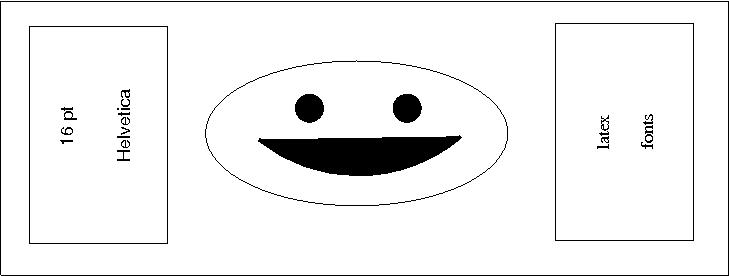
\includegraphics[width=0.9\textwidth]{smile.jpg}
\caption{A jpg}\label{jpg}
\end{figure}

\begin{figure}[!htbp]
\nextalt{This is an alt text for the following png image $4$!}
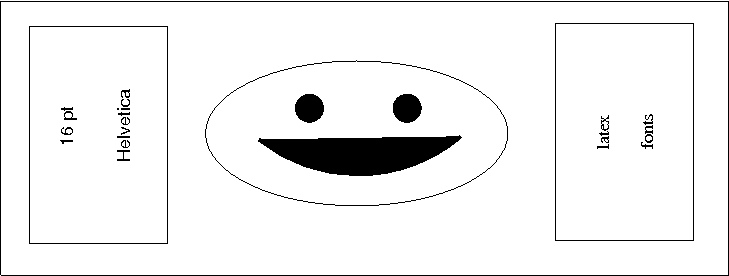
\includegraphics[width=0.9\textwidth]{smile.png}
\caption{A png}\label{png}
\end{figure}

\begin{figure}[!htbp]
\nextalt{This is an alt text for the following pdf image $4$!}
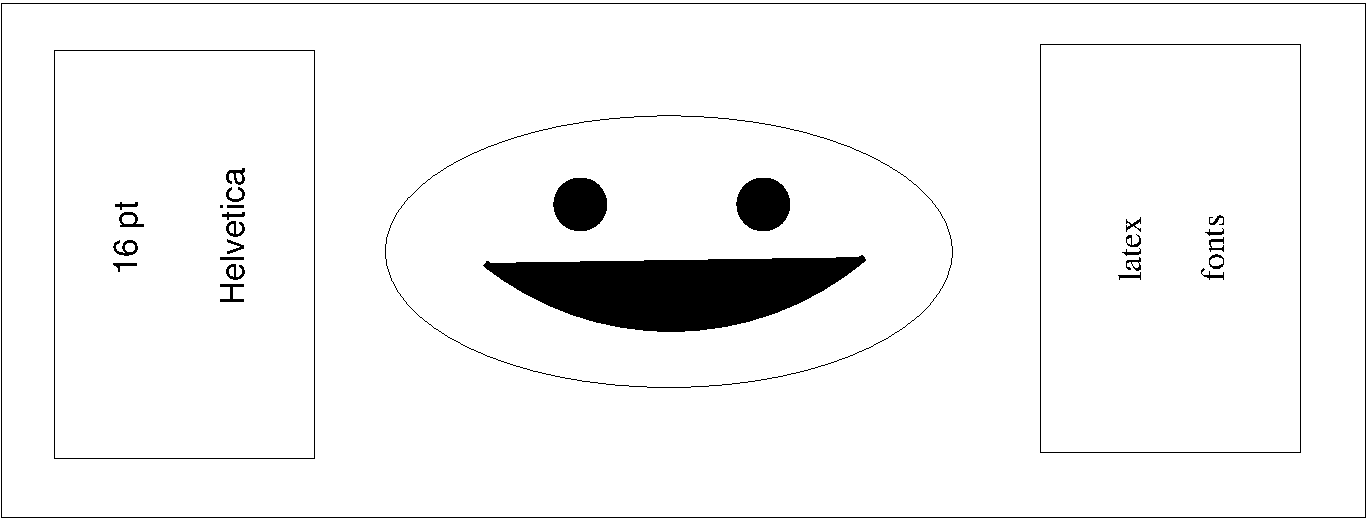
\includegraphics[width=0.9\textwidth]{smile.pdf}
\caption{A pdf}\label{pdf}
\end{figure}

And the last thing I do is to reference an equation I used a long while ago (\ref{alignlab}).

%Diagrams needs to be flushed before the bibliography 
\clearpage

% \thebibliography
\begin{thebibliography}{99}
\bibitem{KopkaDaly} Kopka, H. and Daly, P., \textit{A Guide to \LaTeX}. Pearson Education Ltd., 1999
\end{thebibliography}

\end{document}

